\documentclass[tikz,border=12pt]{standalone}
\usepackage[T1]{fontenc}
\usepackage{lmodern}
\usetikzlibrary{arrows.meta,positioning}
\begin{document}
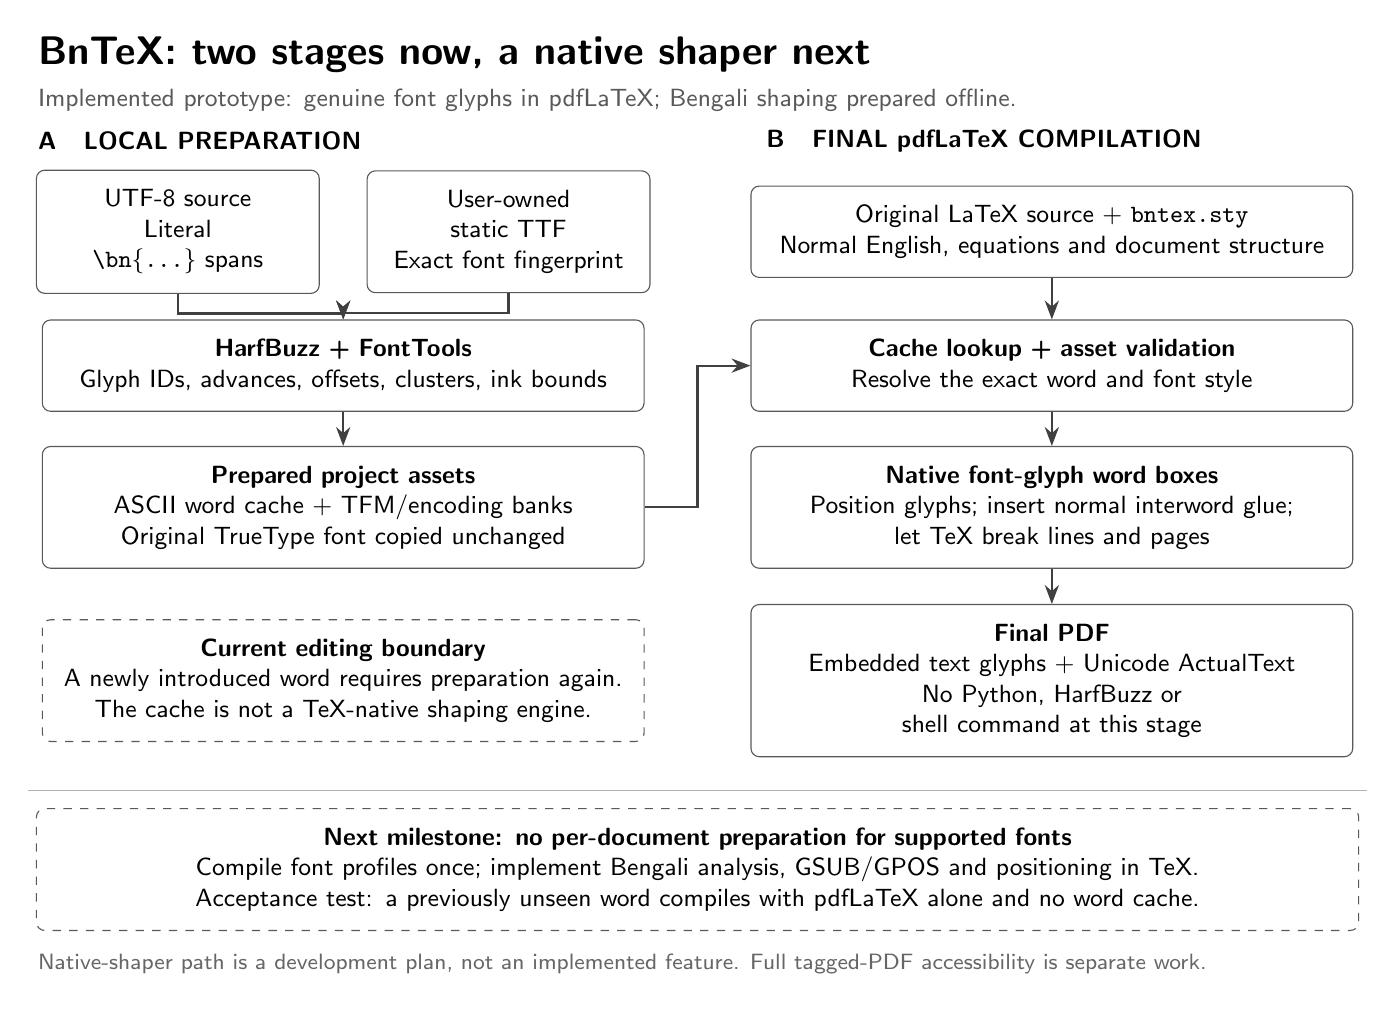
\begin{tikzpicture}[
  font=\sffamily\small,
  box/.style={draw=black!65,rounded corners=3pt,fill=white,align=center,inner sep=7pt,minimum height=1.05cm},
  arrow/.style={-{Stealth[length=2.4mm]},thick,draw=black!75},
  label/.style={font=\sffamily\bfseries\small,anchor=west}
]
\node[anchor=west,font=\sffamily\bfseries\Large] at (0,1.1) {BnTeX: two stages now, a native shaper next};
\node[anchor=west,font=\sffamily\small,text=black!65] at (0,.52)
  {Implemented prototype: genuine font glyphs in pdfLaTeX; Bengali shaping prepared offline.};
\node[label] at (0,0) {A\quad LOCAL PREPARATION};
\node[label] at (9.25,0) {B\quad FINAL pdfLaTeX COMPILATION};
\node[box,text width=3.1cm] (source) at (1.9,-1.15) {UTF-8 source\\Literal \texttt{\string\bn\{...\}} spans};
\node[box,text width=3.1cm] (font) at (6.1,-1.15) {User-owned static TTF\\Exact font fingerprint};
\node[box,text width=7.15cm] (shaper) at (4,-2.85)
  {\textbf{HarfBuzz + FontTools}\\Glyph IDs, advances, offsets, clusters, ink bounds};
\node[box,text width=7.15cm] (assets) at (4,-4.65)
  {\textbf{Prepared project assets}\\ASCII word cache + TFM/encoding banks\\Original TrueType font copied unchanged};
\node[box,dashed,text width=7.15cm] (limit) at (4,-6.85)
  {\textbf{Current editing boundary}\\A newly introduced word requires preparation again.\\The cache is not a TeX-native shaping engine.};
\node[box,text width=7.15cm] (tex) at (13,-1.15)
  {Original LaTeX source + \texttt{bntex.sty}\\Normal English, equations and document structure};
\node[box,text width=7.15cm] (lookup) at (13,-2.85)
  {\textbf{Cache lookup + asset validation}\\Resolve the exact word and font style};
\node[box,text width=7.15cm] (layout) at (13,-4.65)
  {\textbf{Native font-glyph word boxes}\\Position glyphs; insert normal interword glue;\\let TeX break lines and pages};
\node[box,text width=7.15cm] (pdf) at (13,-6.85)
  {\textbf{Final PDF}\\Embedded text glyphs + Unicode ActualText\\No Python, HarfBuzz or shell command at this stage};
\draw[arrow] (source.south) -- ++(0,-.25) -| (shaper.north);
\draw[arrow] (font.south) -- ++(0,-.25) -| (shaper.north);
\draw[arrow] (shaper) -- (assets);
\draw[arrow] (tex) -- (lookup);
\draw[arrow] (lookup) -- (layout);
\draw[arrow] (layout) -- (pdf);
\draw[arrow] (assets.east) -- (8.5,-4.65) -- (8.5,-2.85) -- (lookup.west);
\draw[black!30] (0,-8.25) -- (17,-8.25);
\node[box,dashed,text width=16.3cm,minimum height=1.25cm] at (8.5,-9.25)
  {\textbf{Next milestone: no per-document preparation for supported fonts}\\
   Compile font profiles once; implement Bengali analysis, GSUB/GPOS and positioning in TeX.\\
   Acceptance test: a previously unseen word compiles with pdfLaTeX alone and no word cache.};
\node[anchor=west,font=\sffamily\footnotesize,text=black!60] at (0,-10.45)
  {Native-shaper path is a development plan, not an implemented feature. Full tagged-PDF accessibility is separate work.};
\end{tikzpicture}
\end{document}
